\subsection{Convolution Neural Networks (CNNs) \cite{manilow2020}}

Convolutional Neural Networks (CNNs) are a powerful class of deep learning models renowned for their exceptional performance in image recognition, classification, and other tasks involving grid-like data. Unlike fully connected neural networks, where each node connects to all nodes in the previous layer, CNNs employ a more nuanced architecture inspired by the human visual cortex. This section introduces the key concepts and functionalities of CNNs, highlighting their advantages and potential challenges.

\subsubsection{Convolutional Layers}
The core of a CNN resides in its convolutional layers. These layers consist of nodes that only connect to a small, local region of nodes in the preceding layer. This selective approach offers numerous benefits:

\begin{itemize}
    \item \textbf{Reduced Overfitting:} By limiting connections, CNNs are less susceptible to memorizing training data and more adept at generalizing to unseen examples.
    \item \textbf{Translation Invariance:} CNNs recognize patterns regardless of their location within the input. This invariance is crucial for tasks like object detection, where a cat remains identifiable regardless of its position in an image.
    \item \textbf{Efficient Feature Extraction:} Convolutional layers learn a set of filters (kernels) that slide across the input, detecting specific features like edges, corners, and textures. This feature extraction enables higher-level layers to build upon these basic building blocks for complex pattern recognition.
\end{itemize}

\subsubsection{Key Parameters of CNNs}
The output of a convolutional layer is influenced by four key parameters:

\begin{itemize}
    \item \textbf{Kernel Size:} Determines the dimension and shape of the window that the layer "sees" (Figure \ref{fig:cnn-kernel}). Larger kernels capture broader patterns, while smaller kernels focus on finer details.
    \item \textbf{Stride:} Defines how far the kernel moves between adjacent input nodes. Larger strides reduce the output size but may lose information.
    \item \textbf{Padding:} Controls how the input edges are handled. Padding with zeros or mirrored values maintains the output size while mitigating information loss at the edges (Figure \ref{fig:cnn-padding}).
    \item \textbf{Dilation:} Introduces spaces between the input nodes within the kernel's receptive field (Figure \ref{fig:cnn-dilation}). This allows convolutional nodes to perceive larger contexts without increasing kernel size.
\end{itemize}

\begin{figure} 
    \centering
    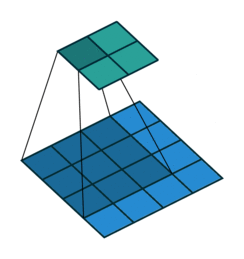
\includegraphics[width=0.25\linewidth]{images/dl/cnn-kernel.png}
    \caption{Convolution with 2D 3x3 filter (kernel) applied on 4x4 input and the output is 2x2. \cite{dumoulin2016guide}}
    \label{fig:cnn-kernel}
\end{figure}

\begin{figure} [h]
    \centering
    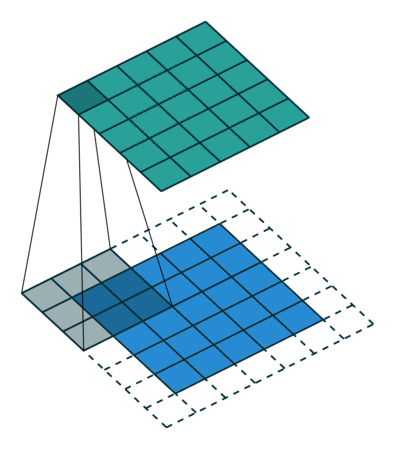
\includegraphics[width=0.25\linewidth]{images/dl/cnn-padding.png}
    \caption{Convolution with 2D 3x3 filter (kernel) applied on 5x5 input with padding 1 and the output is 5x5. \cite{dumoulin2016guide}}
    \label{fig:cnn-padding}
\end{figure}

\begin{figure} [h]
    \centering
    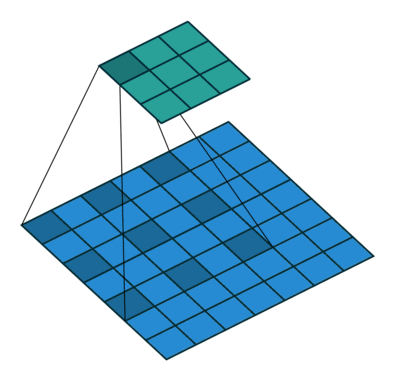
\includegraphics[width=0.25\linewidth]{images/dl/cnn-dilation.png}
    \caption{Dilated Convolution with 2D 3x3 filter (kernel) with dilation factor of 1 applied on 7x7 input  and the output is 3x3. \cite{dumoulin2016guide}}
    \label{fig:cnn-dilation}
\end{figure}

Unlike standard convolutional layers that shrink dimensionality, transpose convolutions (also known as deconvolutional layers) upsample the output. This operation is valuable for tasks like image generation and autoencoders.

Pooling layers further reduce the dimensionality of feature maps by applying functions like max-pooling or average-pooling to non-overlapping sections of the input (Figure \ref{fig:max-pool}). This process retains key information while suppressing redundant details, improving computational efficiency and preventing overfitting.

\begin{figure} [h]
    \centering
    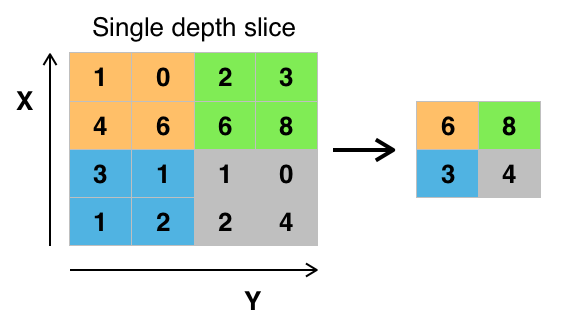
\includegraphics[width=0.75\linewidth]{images/dl/max-pool.png}
    \caption{Max pooling operation applied on a matrix. \cite{dumoulin2016guide}}
    \label{fig:max-pool}
\end{figure}

\subsubsection{CNNs in Audio Processing}
While image recognition remains a primary domain for CNNs, their application extends to audio processing tasks. However, audio data poses unique challenges, as unlike images, sound waves are sequential and lack predefined shapes. To utilize CNNs in audio, data slicing and padding may be necessary to conform to the layer expectations. Edge effects can also arise, potentially distorting the predicted waveform. Overlapping windows, similar to Short-Time Fourier Transform (STFT) computations, can alleviate these issues and improve performance.